\documentclass{beamer}

\mode<presentation>
\usetheme{Madrid}
\definecolor{Columbia}{RGB}{185,217,235}
\definecolor{Columbia2}{RGB}{0,51,160}
\definecolor{Columbia3}{RGB}{0,114,206}
\setbeamercolor{title}{fg=Columbia2}
\setbeamercolor{frametitle}{fg=Columbia2}
\setbeamercolor{block title}{bg=Columbia, fg=Columbia2}
%\setbeamercolor{block body}{fg=Columbia2}
\setbeamercolor{structure}{fg=Columbia}
\setbeamercolor{item projected}{fg=white}
\setbeamercolor{item}{fg=Columbia2}
\setbeamercolor{subitem}{fg=Columbia2}
\setbeamercolor{section in toc}{fg=Columbia}
\setbeamercolor{description item}{fg=Columbia}
\setbeamercolor{caption name}{fg=Columbia}
\usepackage{graphics}
\usepackage{geometry}
\usepackage{booktabs}
\usepackage{multirow, makecell}
\usepackage{float}
\usepackage{fancyvrb}
\usepackage{caption}
\usepackage{subcaption}
\usepackage{adjustbox}
\usepackage{hyperref}

%\hypersetup{
%colorlinks=true,
%linkcolor=black,
%filecolor=green, 
%urlcolor=blue,
%}
\beamertemplatenavigationsymbolsempty
\setbeamertemplate{footline}[page number]
\setbeamercolor{page number in head/foot}{fg=black}
\setbeamertemplate{headline}{}
\makeatletter
\let\@@magyar@captionfix\relax
\makeatother


\title[Econometrics 2]{Introduction to Econometrics 2: Recitation 9} % Change this regularly
\author{Seung-hun Lee}
\institute{Columbia University}

\date{April 8th, 2020}

\begin{document}
\begin{frame}
\titlepage
\end{frame}


\begin{frame}
\frametitle{Quantile Regression}
Motivation
\begin{itemize}
\item The usual linear regression, which has the form
\[
y= X\beta+u
\]
where $E(Xu)=0$ (or more restrictively, $E(u|X)=0$)
\item This setup is aimed at capturing the conditional mean of $y$ given $X$. 
\item However, there is no reason to restrict our attention to just a conditional mean. We might want a conditional median etc.
\item  \textbf{Quantile regression} aims to capture different values of $\beta$ depending on the location of the conditional distribution.
\end{itemize}
\end{frame}

\begin{frame}
\frametitle{Quantile Regression}
Setup
\begin{itemize}
\item The quantile regression seeks to estimate the conditional quantile
\[
q_\tau(y | X)=X\beta_\tau
\]
where $\tau\in[0,1]$ is the percentile of our choice satisfying $F_{y|X}(X\beta_\tau|X)=\tau$.
\item With
\[
F_{y|X}(X\beta_\tau|X)=\Pr(y\leq X\beta_\tau|X)=\tau
\]
we can write 
\[
\tau-\Pr(y\leq X\beta_\tau|X)=0
\]
Since $\Pr(y\leq X\beta_\tau|X)$ is equal to $E[1(y- X\beta_\tau\leq 0)]=E[1(u\leq0)]$, we can obtain the condition
\[
E[\tau-1(y- X\beta_\tau\leq 0)|X]=0
\]
this also implies $E[(\tau-1(y- X\beta_\tau\leq 0))X]=0$
\end{itemize}
\end{frame}

\begin{frame}
\frametitle{Quantile Regression}
Setup: Check Function
\begin{itemize}
\item The check function can be defined as
\[
\rho_\tau(u)=u(\tau-1(u\leq0))
\]
\begin{itemize}
\item Median: Let $\tau=1/2$. Then the check function becomes
\[
\rho_{1/2}(u)=\begin{cases}-\frac{1}{2}u & (u\leq 0) \\ \frac{1}{2}u & (u>0) \end{cases} = \frac{1}{2}|u|=\frac{1}{2}|y-X\beta_{1/2}|
\]
This becomes equivalent to solving the least absolute deviation problem.
\item $\tau=1/3$: Then the check function becomes
\[
\rho_{1/3}(u)=\begin{cases}-\frac{2}{3}u & (u\leq 0) \\ \frac{1}{3}u & (u>0) \end{cases}
\]
which has a kink at $u=0$ and is asymmetric.
\end{itemize}
\end{itemize}
\end{frame}

\begin{frame}
\frametitle{Quantile Regression}
Finding the Quantile Estimator
\begin{itemize}
\item The minimization problem solved in quantile regression is
\[
\min_\beta E[ \rho_\tau(y-X\beta_\tau)|X]
\]
which can be written as
\footnotesize{\begin{align*}
E[ \rho_\tau(y-X_i\beta_\tau)|X] &= (\tau-1)\int_{-\infty}^{a} (y-a)f_{Y|X}(y|x)dy+ \tau\int_{a}^\infty(y-a) f_{Y|X}(y|x)dy\\
\end{align*}}\normalsize
where $a=X\beta_\tau$
\item Take the first order condition w.r.t. $a$ to get
\begin{gather*}
-(\tau-1)\int_{-\infty}^a f_{Y|X}(y|x)dy - \tau\int_a^\infty f_{Y|X}(y|x)dy=0\\
\iff -\tau + F(a|X)=0
\end{gather*}
\end{itemize}
\end{frame}

\begin{frame}
\frametitle{Quantile Regression}
Finding the Quantile Estimator
\begin{itemize}
\item Thus, the $\beta_\tau$ that solves
\[
X\beta_\tau=a=F^{-1}_{Y|X}(\tau|X)
\]
is the $\beta_\tau$ that we are looking for
\item We can also solve for
\[
\min_\beta E[\rho_\tau(y-X\beta_\tau)X]
\] 
or in a sample analogue
\[
\min_\beta \frac{1}{n}\sum_{i=1}^n \rho_\tau(y_i-X_i\beta_\tau)X_i
\]
\item For suitable conditions, the resulting estimator is CAN.
\end{itemize}
\end{frame}

\begin{frame}
\frametitle{Quantile Regression}
Examples
\begin{itemize}
\item Levin (2001)
\begin{itemize}
\item In educational production function literature, the effect of class size on various outcomes for the student is controversial 
\item Uses quantile regression in estimating educational production
\item Also controls for peer effects - turns out that this effect matters more especially for those in the low achievement group
\item Class size does not have as significant effect
\end{itemize}
\item Autor, Houseman, Kerr (2017)
\begin{itemize}
\item Studies effect of direct hire assistance and temporary-help job placement programs in Detroit on distribution of participant's earnings over a 7-quarter period
\item For low-tail, none are effective. For high-tail, direct hire raises earnings but temporary-help does not
\item Autor, Houseman (2010) study the same program without QR and finds on avg that earnings increased
\end{itemize}
\end{itemize}
\end{frame}


\begin{frame}
\frametitle{Nonparametric Regression}
Motivation
\begin{itemize}
\item Consider a setting where we observe the data $(y_i,x_i)$ which is i.i.d. and drawn from a DGP $P_0(y|x)$.
\item We are interested in backing out the whole or part of the data generating process $P_0(y|x)$ \textbf{without any modeling assumptions}
\item This approach is called a \textbf{nonparametric} approach
\item We normally use nonparametric approach to 
\begin{itemize}
\item Conduct a diagnostic checking of an estimated parametric model, 
\item To conveniently display key features of the dataset 
\item Conduct an inference under very weak assumptions.
\end{itemize}
\end{itemize}
\end{frame}

\begin{frame}
\frametitle{Nonparametric Regression}
Idea
\begin{itemize}
\item For discrete-valued $Y$ and $X$, this is relatively easy. Just back out the data generating process of interest
\[
\hat{P}(y\in A| x\in B)=\frac{n^{-1}\sum_{i=1}^n1(y_i\in A, x_i\in B) }{n^{-1}\sum_{i=1}^n1(x_i\in B)}
\]
Provided that $P_0(x\in B)\neq 0$, then the above estimator converges to the true $P_0(y|x)$ as $n\to\infty$.
\item For continuous cases, $A\equiv (-\infty, y], B\equiv[x-\epsilon, x+\epsilon]$ and use $\lim_{\epsilon\to0}\hat{P}(A|B)$ to back out the DGP
\item  This can be problematic when we have too many dimensions of $X$
\item Therefore, the method to conduct nonparametric estimation in this context is kernel density function approach. 
\end{itemize}
\end{frame}

\begin{frame}
\frametitle{Nonparametric Regression}
Kernels
\begin{itemize}
\item Consider the problem of estimating the probability density function $f(x)$ of a random scalar variable $X$ at $X=x$
\item  Let $\{X_1,...,X_n\}$ be a random sample of $X$. If $f$ is a smooth function, we can approximate $f$ by
\[
f(x)\simeq \frac{\int_{x-h}^{x+h}f(u)du}{2h}
\]
for a small $h$
\item The numerator on the right hand side can be estimated using a sample analogue of the following form
\[
\frac{1}{n}\sum_{i=1}^n 1\{x-h\leq X_i \leq x+h \}
\]
\end{itemize}
\end{frame}

\begin{frame}
\frametitle{Nonparametric Regression}
Kernels
\begin{itemize}
\item Combining the two expressions, we can approximate $f(x)$ with
\footnotesize{\begin{align*}
\hat{f}(x)&=\frac{n^{-1}\sum_{i=1}^n 1[x-h\leq X_i \leq x+h]}{2h} \\
&=\frac{1}{2nh}\sum_{i=1}^n 1[x-h\leq X_i \leq x+h]\\
&=\frac{1}{nh}\sum_{i=1}^n \frac{1}{2}1\left[\left|\frac{x-X_i}{h}\right| \leq 1\right]\\
&=\frac{1}{nh}\sum_{i=1}^n K\left(\frac{x-X_i}{h}\right)
\end{align*}}\normalsize
where $K(u)=\frac{1}{2}1(|u|\leq 1)$ - a uniform kernel. 
\item $K(\cdot)$ is a \textbf{kernel density estimator}. It should be a real-to-real function, positive and smooth and integrates to 1 on its support
\item Generally type of kernels rarely matter
\end{itemize}
\end{frame}

\begin{frame}
\frametitle{Nonparametric Regression}
Bandwidth
\begin{itemize}
\item However, bandwidths do matter, as they are involved in the the trade-off between bias and variance
\begin{figure}[H]
\centering
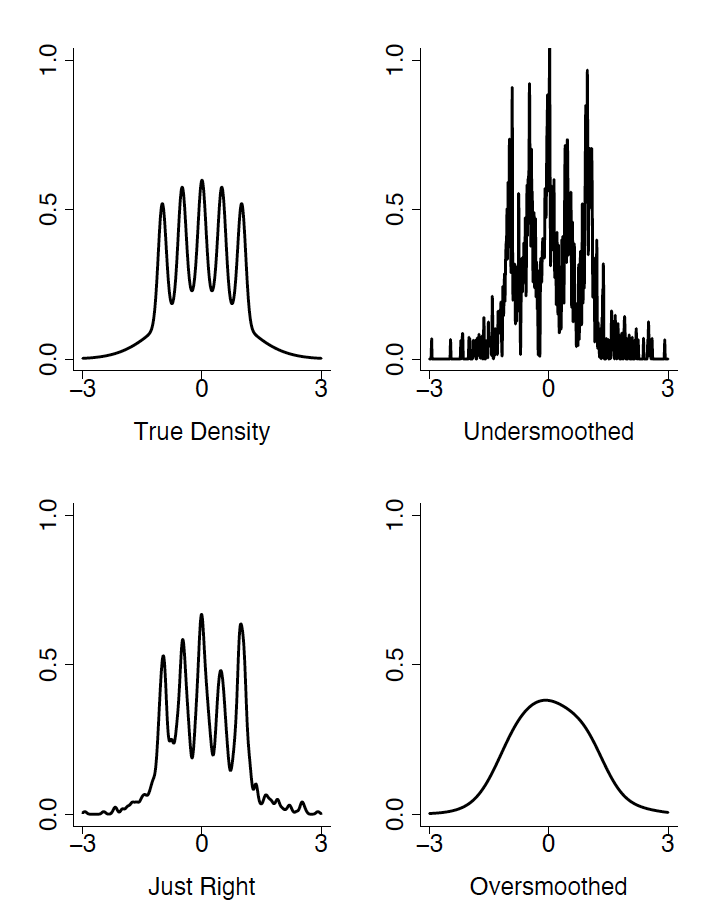
\includegraphics[height=0.75\textheight, keepaspectratio]{smoothing.png}
\end{figure}
\end{itemize}
\end{frame}

\begin{frame}
\frametitle{Nonparametric Regression}
Bandwidth: Characterizing Bias
\footnotesize{\begin{align*}
E[\hat{f}(x)]&=\frac{1}{h}\int_{-\infty}^\infty K\left(\frac{x-s}{h}\right)f(s)ds\\
&=-\frac{1}{h}\int_{-\infty}^\infty K(t)f(x-ht)(-hdt) \ (\because \frac{x-s}{h}=t \ \text{transformation})\\
&=\int_{-\infty}^\infty K(t)f(x-ht)dt\\
&=\int_{-\infty}^\infty K(t)\left[f(x)-f'(x)ht + \frac{f''(x)h^2t^2}{2}+o(h^2)\right]dt\\
&=f(x)-0+\frac{1}{2}\int_{-\infty}^\infty K(t)h^2t^2f''(x)dt + o(h^2)
\end{align*}}\normalsize
Where $\int_{-\infty}^\infty K(t)dt=1$ justifies $f(x)$ and $\int_{-\infty}^\infty tK(t)dt=0$ (since kernel is symmetric around 0) justifies second term in the last line being 0
\begin{itemize}
\item Thus, bias is
\[
E[\hat{f}(x)]-f(x)=\frac{1}{2}\int_{-\infty}^\infty K(t)h^2t^2f''(x)dt
\]
\end{itemize}
\end{frame}

\begin{frame}
\frametitle{Nonparametric Regression}
Bandwidth: Characterizing Variance
\scriptsize{\begin{align*}
Var[\hat{f}(x)]&=E\left[\frac{1}{n^2h^2}\left(\sum_{i=1}^nK\left(\frac{x-X_i}{h}\right)\right)^2\right]-(E[\hat{f}(x)])^2\\
&=E\left[\frac{1}{n^2h^2}\left(\sum_{i=1}^nK^2\left(\frac{x-X_i}{h}\right)+2\sum_{i<j} K\left(\frac{x-X_i}{h}\right)K\left(\frac{x-X_j}{h}\right)\right)\right]-(E[\hat{f}(x)])^2\\
&=\frac{1}{nh^2}\int_{-\infty}^\infty K^2\left(\frac{x-s}{h}\right)f(s)ds+\frac{n(n-1)}{n^2h^2}\left(\int_{-\infty}^\infty K\left(\frac{x-s}{h}\right)f(s)ds\right)^2\\
&-\frac{1}{h^2}\left(\int_{-\infty}^\infty K\left(\frac{x-s}{h}\right)f(s)ds\right)^2
 \end{align*}}\normalsize
Then, use variable transformation and Taylor approximation. 
\begin{itemize}
\item Thus, the leading term of bias is 
\[
\frac{1}{nh}\int_{-\infty}^\infty K^2(t)f(x)dt\simeq O\left(\frac{1}{nh}\right)
\]
\item So low $h$ drops bias at the expense of rising variance
\end{itemize}
\end{frame}

\begin{frame}
\frametitle{Nonparametric Regression}
Optimal Bandwidth?
\begin{itemize}
\item Optimal $h$ minimizes the loss function, or asymptotic mean integrated squared error (AMISE), defined as
 \[
 \int E(\hat{f}(x)-f(x))^2dx
 \]
\item We can show that $MSE=\text{Variance+Bias}^2$
\item From the discussion about the variance and bias, 
 \footnotesize{\begin{align*}
 \text{Variance}+\text{Bias}^2=\frac{1}{nh}\int_{-\infty}^\infty K^2(t)f(x)dt+\frac{h^4}{4}(f''(x))^2\left(\int_{-\infty}^\infty K(t)t^2dt\right)^2
 \end{align*}}\normalsize
\item  Thus, the final version of AMISE can be written as
 \footnotesize{\[
 \int(\text{Variance}+\text{Bias}^2)dx=\frac{1}{nh}\int_{-\infty}^\infty K^2(t)dt+\frac{h^4}{4}\int_{-\infty}^\infty(f''(x))^2\left(\int_{-\infty}^\infty K(t)t^2dt\right)^2 dx
 \]}\normalsize
\end{itemize}
\end{frame}

\begin{frame}
\frametitle{Nonparametric Regression}
Optimal Bandwidth?
\begin{itemize}
\item If  $A=\frac{1}{4}\int_{-\infty}^\infty(f''(x))^2\left(\int_{-\infty}^\infty K(t)t^2dt\right)^2 dx$, $B=\int_{-\infty}^\infty K^2(t)dt$. Then
 \[
 AMISE =Ah^4+\frac{B}{nh}
 \]
\item Then, the minimization problem becomes $\min_h AMISE$. Therefore, we find $h$ satisfying
 \[
 4Ah^3-Bn^{-1}h^{-2}=0\iff h^5=\frac{B}{4An} \iff h=\left(\frac{B}{4An}\right)^{1/5}
 \]
 \begin{itemize}
\item In this framework, the bias and standard errors are both in $n^{-2/5}$ and AMISE will be in $n^{-4/5}$. Therefore, we may not have a CAN estimator at $n^{-1/2}$
\item Even bigger problem arises from $\int f''(x)dx$ term in $A$, as we are not sure of $f(x)$ to begin with, we do not know what $f''(x)$ would be.
\end{itemize}
\end{itemize}
\end{frame}

\begin{frame}
\frametitle{Nonparametric Regression}
Bandwidth Choice in Practice
\begin{itemize}
\item Silverman: Use $1.06\sigma n^{-1/5}$ for a normal kernel
\item Robust version: $ h=0.9 \min\{s,IQ/1.34\}n^{-1/5}$
\item Cross Validation: Use a leave-one-out estimator defined as
 \[
 \hat{f}_{-i}(x) = \frac{1}{nh}\sum_{j\neq i}K\left(\frac{x-x_j}{h}\right)
 \]
 \item Local bandwidth: Make $h$ larger in a low density area (decrease variance). In a wiggly region, it is better to take $h$ smaller. (minimize biases). 
\end{itemize}
\end{frame}

\begin{frame}
\frametitle{Nonparametric Regression}
Curse of Dimensionality
\begin{itemize}
\item  Now assume that $x$ is not necessarily a scalar, but of dimension $d$. 
\item Then we can use a $d$-dimensional kernel $K$ and estimate $f(x)$ with
 \[
 \hat{f}(x)= \frac{1}{nh^d}\sum_{i=1}^nK\left(\frac{x-x_i}{h}\right)
 \]
 where $K$ can be a $d$-product of a uni-dimensional kernels
 \item Not necessarily confined to using a same bandwith for all $d$ kernels.
\item We may want to sphericize if the kernel estimators are correlated.
\item  A bigger concern has to do with the computation cost from using a large $d$ - a \textbf{curse of dimensionality}
\end{itemize}
\end{frame}

\begin{frame}
\frametitle{Nonparametric Regression}
Curse of Dimensionality
\begin{itemize}
\item Return to calculating $E[\hat{f}(x)^2]$ term in AMISE, 
 \footnotesize{\begin{align*}
 E[\hat{f}(x)^2]&=E\left[\frac{1}{n^2h^{2d}}\left(\sum_{i=1}^nK\left(\frac{x-X_i}{h}\right)\right)^2\right]\\
 &=E\left[\frac{1}{n^2h^{2d}}\left(\sum_{i=1}^nK^2\left(\frac{x-X_i}{h}\right)+2\sum_{i<j} K\left(\frac{x-X_i}{h}\right)K\left(\frac{x-X_j}{h}\right)\right)\right]\\
 &=\frac{1}{nh^{2d}}\int_{-\infty}^\infty K^2\left(\frac{x-s}{h}\right)f(s)ds+\frac{n(n-1)}{n^2h^{2d}}\left(\int_{-\infty}^\infty K\left(\frac{x-s}{h}\right)f(s)ds\right)^2
 \end{align*}}\normalsize
 \item The leading term is
\footnotesize{ \[
\frac{1}{nh^{2d}}\int_{-\infty}^\infty K^2\left(\frac{x-s}{h}\right)f(s)ds \simeq \frac{1}{nh^d}\int K^2(t)f(x-ht)dt = O\left(\frac{1}{nh^d}\right)
 \]}\normalsize
\item The optimal $h$ will be in $n^{-\frac{1}{4+d}}$ and convergence occurs in $n^{-\frac{2}{4+d}}$ - at an even slower rate. So more $n$ required to guarantee precision. 
\end{itemize}
\end{frame}

\begin{frame}
\frametitle{Nonparametric Regression}
Nadaraya-Watson Estimation
\begin{itemize}
\item Given the data $(y_i,x_i)$, we are attempting to capture $E[g(y,x)|x]=m(x)$ for some $g(y,x)$. 
\item For instance, we can attempt to estimate the conditional expectation by letting $g(y,x)=y$. 
\item Note that the conditional expected value can be written as
 \begin{align*}
 E[y|x]&=\int y f_{Y|X}(y|x)dy \\
 &=\int y \frac{f_{Y,X}(y,x)}{f_{X}(x)}dy=\frac{\int yf_{Y,X}(y,x)dy}{\int f_{Y,X}(y,x)dy}
 \end{align*}
\item  We can obtain the nonparametric estimator for the conditional expected value by replacing $f_{Y,X}$ with its kernel estimator
\end{itemize}
\end{frame}

\begin{frame}
\frametitle{Nonparametric Regression}
Nadaraya-Watson Estimation
\begin{itemize}
\item  The numerator becomes
 \footnotesize{\begin{align*}
 \int y \hat{f}(y,x)dy&=\int y \frac{1}{nh^2}\sum_{i=1}^n K\left(\frac{x-X_i}{h}\right)K\left(\frac{y-Y_i}{h}\right)dy\\
 &= \frac{1}{nh^2}\sum_{i=1}^n K\left(\frac{x-X_i}{h}\right)\int yK\left(\frac{y-Y_i}{h}\right)dy\\
 &=\frac{1}{nh^2}\sum_{i=1}^n K\left(\frac{x-X_i}{h}\right)\int (Y_i+sh)K\left(s\right)(hds) \ (\because s=\frac{y-Y_i}{h})\\
 &= \frac{1}{nh}\sum_{i=1}^n K\left(\frac{x-X_i}{h}\right)Y_i\ (\because \int K(s)ds=1, \int sK(s)ds=0)
 \end{align*}}\normalsize
 \item The denominator can be written as $ \frac{1}{nh}\sum_{i=1}^n K\left(\frac{x-X_i}{h}\right)$. Thus, the estimator for the conditional expectation becomes
 \[
 \frac{\sum_{i=1}^n Y_iK\left(\frac{x-X_i}{h}\right)}{\sum_{i=1}^n K\left(\frac{x-X_i}{h}\right)}
 \]
\end{itemize}
\end{frame}

\begin{frame}
\frametitle{Nonparametric Regression}
Nadaraya-Watson Estimation
\begin{itemize}
\item  Effectively we are putting weight $\frac{K\left(\frac{x-X_i}{h}\right)}{\sum_{i=1}^nK\left(\frac{x-X_i}{h}\right)}$ on each observation 
\item This is also a \textbf{local constant estimation} in the sense that when solving the following minimization problem
 \[
 \hat{f}(x)=\arg\min_a\frac{1}{nh}\sum_{i=1}^n(Y_i-a)^2K\left(\frac{x-X_i}{h}\right)
 \]
 The first order condition on $a$ yields the following results
 \[
 \sum_{i=1}^nY_iK\left(\frac{x-X_i}{h}\right)=a\sum_{i=1}^nK\left(\frac{x-X_i}{h}\right) \implies a= \frac{\sum_{i=1}^n Y_iK\left(\frac{x-X_i}{h}\right)}{\sum_{i=1}^n K\left(\frac{x-X_i}{h}\right)}
 \]
\item  As for the optimal $h$, it is possible to use cross-validation method and minimizing AMISE. 
\item This method can be unreliable if $f(x)\to0$
\end{itemize}
\end{frame}

\begin{frame}
\frametitle{Nonparametric Regression}
Nadaraya-Watson Estimation
\begin{itemize}
\item  We can also do something more general. e.g. \textbf{local linear estimation}. 
\item We regress $g(y,x)$ on a constant ($a$) and a linear term ($b(x-X_i)$).
\item In mathematical expression, we solve
 \[
 \min_{a,b}\frac{1}{nh}\sum_{i=1}^n(Y_i-a-b(x-X_i))^2K\left(\frac{x-X_i}{h}\right)
 \]
 and obtain that $\hat{a}=\hat{g}$ and $\hat{b}$ is an estimate of $\frac{\partial g(x)}{\partial x}$.
 \item If it happens that the true functional form is linear, then this estimate does not produce a bias.
 \item In addition, local linear estimation performs better than local constant estimation in the boundaries of the support for $X$. \par
 \item We can do even more with \textbf{local polynomial estiation} by regressing $g(y,x)$ on a constant, $x-X_i$, $(x-X_i)^2$ and so on. 
\end{itemize}
\end{frame}

\begin{frame}
\frametitle{Nonparametric Regression}
Semi-nonparametric Estimation
\begin{itemize}
\item Suppose that we are sure that $f(x)$ can be characterized by $f_{m,\sigma}$ where $m,\sigma$ indexes some properties of the density function $f$. 
\item Then, by Weierstrass approximation theorem, we can choose a family of positive functions which increases in complexity $P_\theta^1, P_\theta^2,...$ and maximize over the loglikelihood
\[
\sum_{i=1}^n \log{f_{m,\sigma}(X_i)}P_\theta^M(X_i)
\]
\item Mixture of normals: Suppose that $Y|X$ is drawn from the two distributions
\begin{itemize}
\item $N_1(m_1(x,\theta), \sigma_1^2(x,\theta))$ with probability $q_1(x,\theta)$
\item $N_2(m_2(x,\theta). \sigma_2^2(x,\theta))$ with probability $q_2(x,\theta)$
\end{itemize}
Then, we apply a maximum likelihood of the following form
\footnotesize{\[
\min_\theta \sum_i\sum_k q_k(x_i,\theta)[(y_i-m_k(x_i,\theta))'\sigma_k(x_i,\theta)^{-1}(y_i-m_k(x_i,\theta))+\log\det{\sigma_k(x_i,\theta)}]
\]}\normalsize
\end{itemize}
\end{frame}

\begin{frame}
\frametitle{Nonparametric Regression}
Semi-nonparametric Estimation: Series Estimation
\begin{itemize}
\item Let $\{P_k(x_i)|k=1,2...\}$ be the orthonormal basis for a smooth function.
\begin{itemize}
\item $\int P_k(x)^2 dx=1, \int P_k(x) P_m(x)=0 \ (k\neq m)$
\end{itemize}
\item These could be polynomials of degree $k$, sine functions and so on.
\item Run a linear regression that has the following form
\[
y_i = \sum_{k=1}^MP_k(x_i)\theta_k+\epsilon_i
\]
\item The $\sum_{k=1}^MP_k(x_i)\theta_k$ part is a series approximation to $g(x)$. 
\item However, depending on the number of $M$ that we choose, the curse of dimensionality can kick in. 
\end{itemize}
\end{frame}
%%%%%%%%%%%
\end{document}
